\section{Trombe Walls }\label{trombe-walls}

Trombe walls are passive solar devices designed for thermal storage and delivery.~ It consists of a thick wall (150mm to 300mm) {[}8" to 16"{]} faced with a selective surface solar absorber, air gap, and high transmissivity glass pane.~ Trombe walls are usually South facing (in the Northern Hemisphere) for maximum sun exposure.~ An overhang above the wall is used to decrease exposure in the summer when the sun is high in the sky and heating is not required, yet still allows for full exposure in the winter when the sun is low in the sky and heating is desirable.

In EnergyPlus, there is no Trombe wall object per se; rather, it is composed of other existing EnergyPlus objects in the input file (except for a special key choice for Zone Inside Convection Algorithm in the Zone input object).~ This approach provides flexibility in specifying the various wall parameters and allows the freedom to explore unusual configurations.~ On the other hand, this approach puts more of a burden on the user to be sure that all parts of the Trombe wall are correctly specified; otherwise unexpected results may be obtained.

To simulate the Trombe wall, a very narrow zone is coupled to the desired surface via an interzone partition.~ The depth of the zone corresponds to the size of the air space usually 18mm to 150mm (¾" to 6").~ In most cases the Trombe zone will be a sealed zone with no ventilation.~ The exterior wall of the Trombe zone contains a single or double-pane window.~ Optimally, the window covers nearly all of the wall area and has a very high transmissivity to allow the maximum amount of solar flux into the Trombe zone.~ Frames and dividers can be defined as usual for the window.~ The interior wall is usually constructed of very thick masonry materials with a solar absorber surface as the innermost layer of the wall.~ The absorber is a selective surface material with very high absorptivity and very low emissivity, e.g.~copper with a special black surface treatment.~ It is important to make sure the Solar Distribution field in the \textbf{Building} object is set to FullInteriorAndExterior so that the majority of the solar flux is directed on the absorber surface and not just on the very small area of the Trombe zone floor. ~The Zone Inside Convection Algorithm for the Trombe's Zone object should also be set to TrombeWall to correctly model the air space.~ As is the case for all interzone partitions, the wall construction of the adjoining zone must be the mirror image of the wall construction in the Trombe zone.~ Finally, an overhang is optionally attached to the Trombe zone to control the amount of seasonal sun exposure.~ Since the user selects all of the Trombe wall parameters in the input file, there is considerable freedom to experiment with different materials, sizes, and configurations.

\begin{figure}[hbtp] % fig 307
\centering
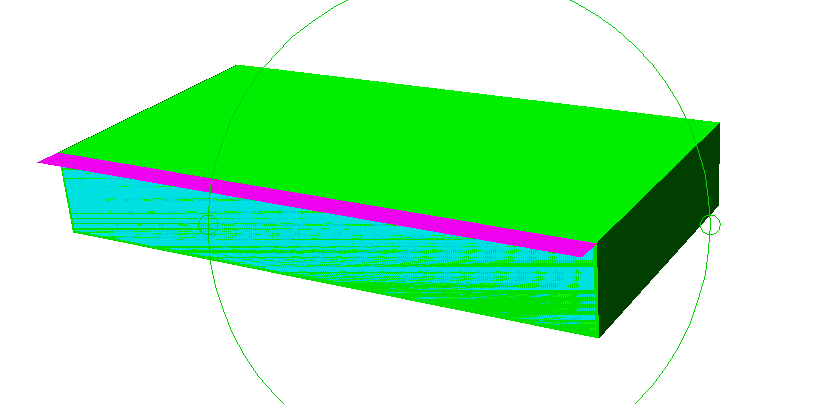
\includegraphics[width=0.9\textwidth, height=0.9\textheight, keepaspectratio=true]{media/image6830.png}
\caption{Building with Trombe Wall \protect \label{fig:building-with-trombe-wall}}
\end{figure}

\subsection{Passive Trombe Wall}\label{passive-trombe-wall}

Passive Trombe walls perform without the assistance of any additional mechanical equipment.~ Most Trombe walls are passive Trombe walls.~ They can be either sealed or naturally ventilated.

For a sealed or unvented Trombe wall, the \emph{Zone Inside Convection Algorithm} field in the Zone object should be set to ``TrombeWall''.~ This algorithm correctly calculates the convection coefficients for a narrow sealed vertical cavity based on the ISO 15099 standard.~ Refer to the ``Trombe Wall Algorithm'' subsection (under Interior Convection, above) for a complete description of the algorithm.~ The EnergyPlus modeling approach for the sealed passive Trombe wall has been validated with experimental data (Ellis 2003).

For a naturally ventilated Trombe wall, there is no built-in algorithm for calculating the correct convection coefficients on the inside of the cavity walls.~ One option is to use the ``Detailed'' convection algorithm.~ This algorithm takes into account some natural convection effects but is intended for a normal sized room.~ Therefore, some error may be incurred when used with a narrow cavity.~ Another option is to use the SurfaceProperty:ConvectionCoefficients object to schedule coefficients that have been determined beforehand by the user.

\subsubsection{Input File}\label{input-file}

An input file (PassiveTrombeWall.idf) is provided to demonstrate a sample sealed Trombe wall implementation.~ In this file two separated fictional buildings are simulated for summer and winter design days in Zion, Utah.~ The buildings are identical in size and construction except that one has a Trombe wall and the other does not.~ The buildings have uncontrolled zones with no internal loads and heavy insulation.~ All floors use interzone partitions to disconnect them from the ground.~ The window on the Trombe zone is a 3 mm, low iron, single pane glazing with very high transmissivity (0.913 visible, 0.899 solar).~ The absorber surface is a Tabor solar absorber with an emittance of 0.05 and absorptance of 0.85.

\subsubsection{Results}\label{results-000}

The resulting temperature profiles for winter and summer design days are plotted below.

\begin{figure}[hbtp] % fig 308
\centering
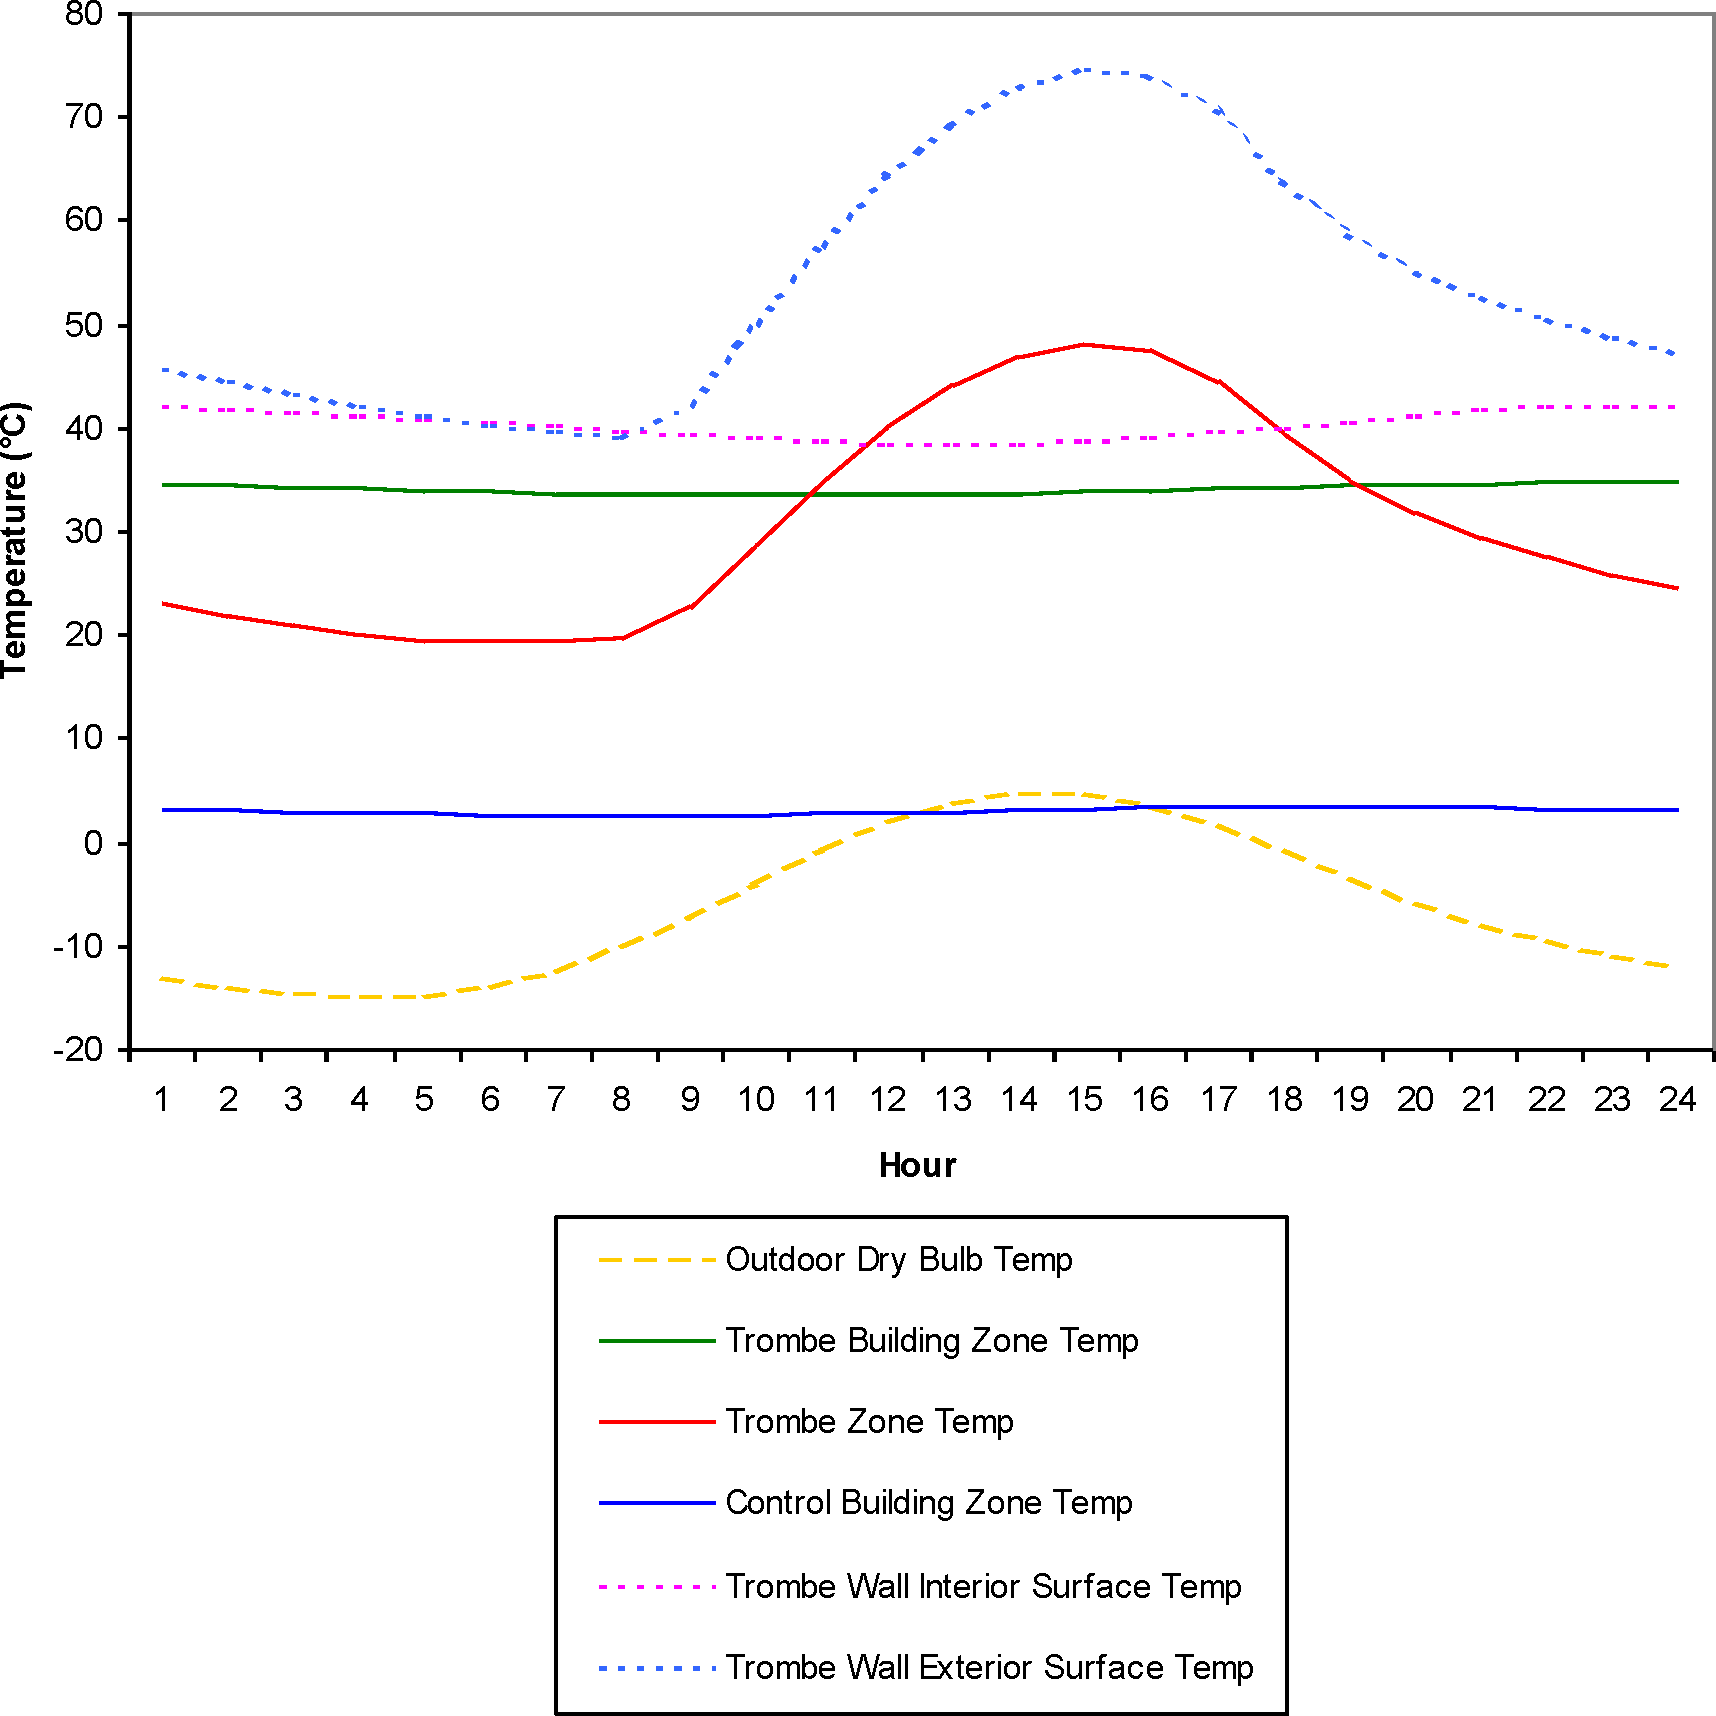
\includegraphics[width=0.9\textwidth, height=0.9\textheight, keepaspectratio=true]{media/image6831.png}
\caption{Passive Trombe Wall Winter \protect \label{fig:passive-trombe-wall-winter}}
\end{figure}

\begin{figure}[hbtp] % fig 309
\centering
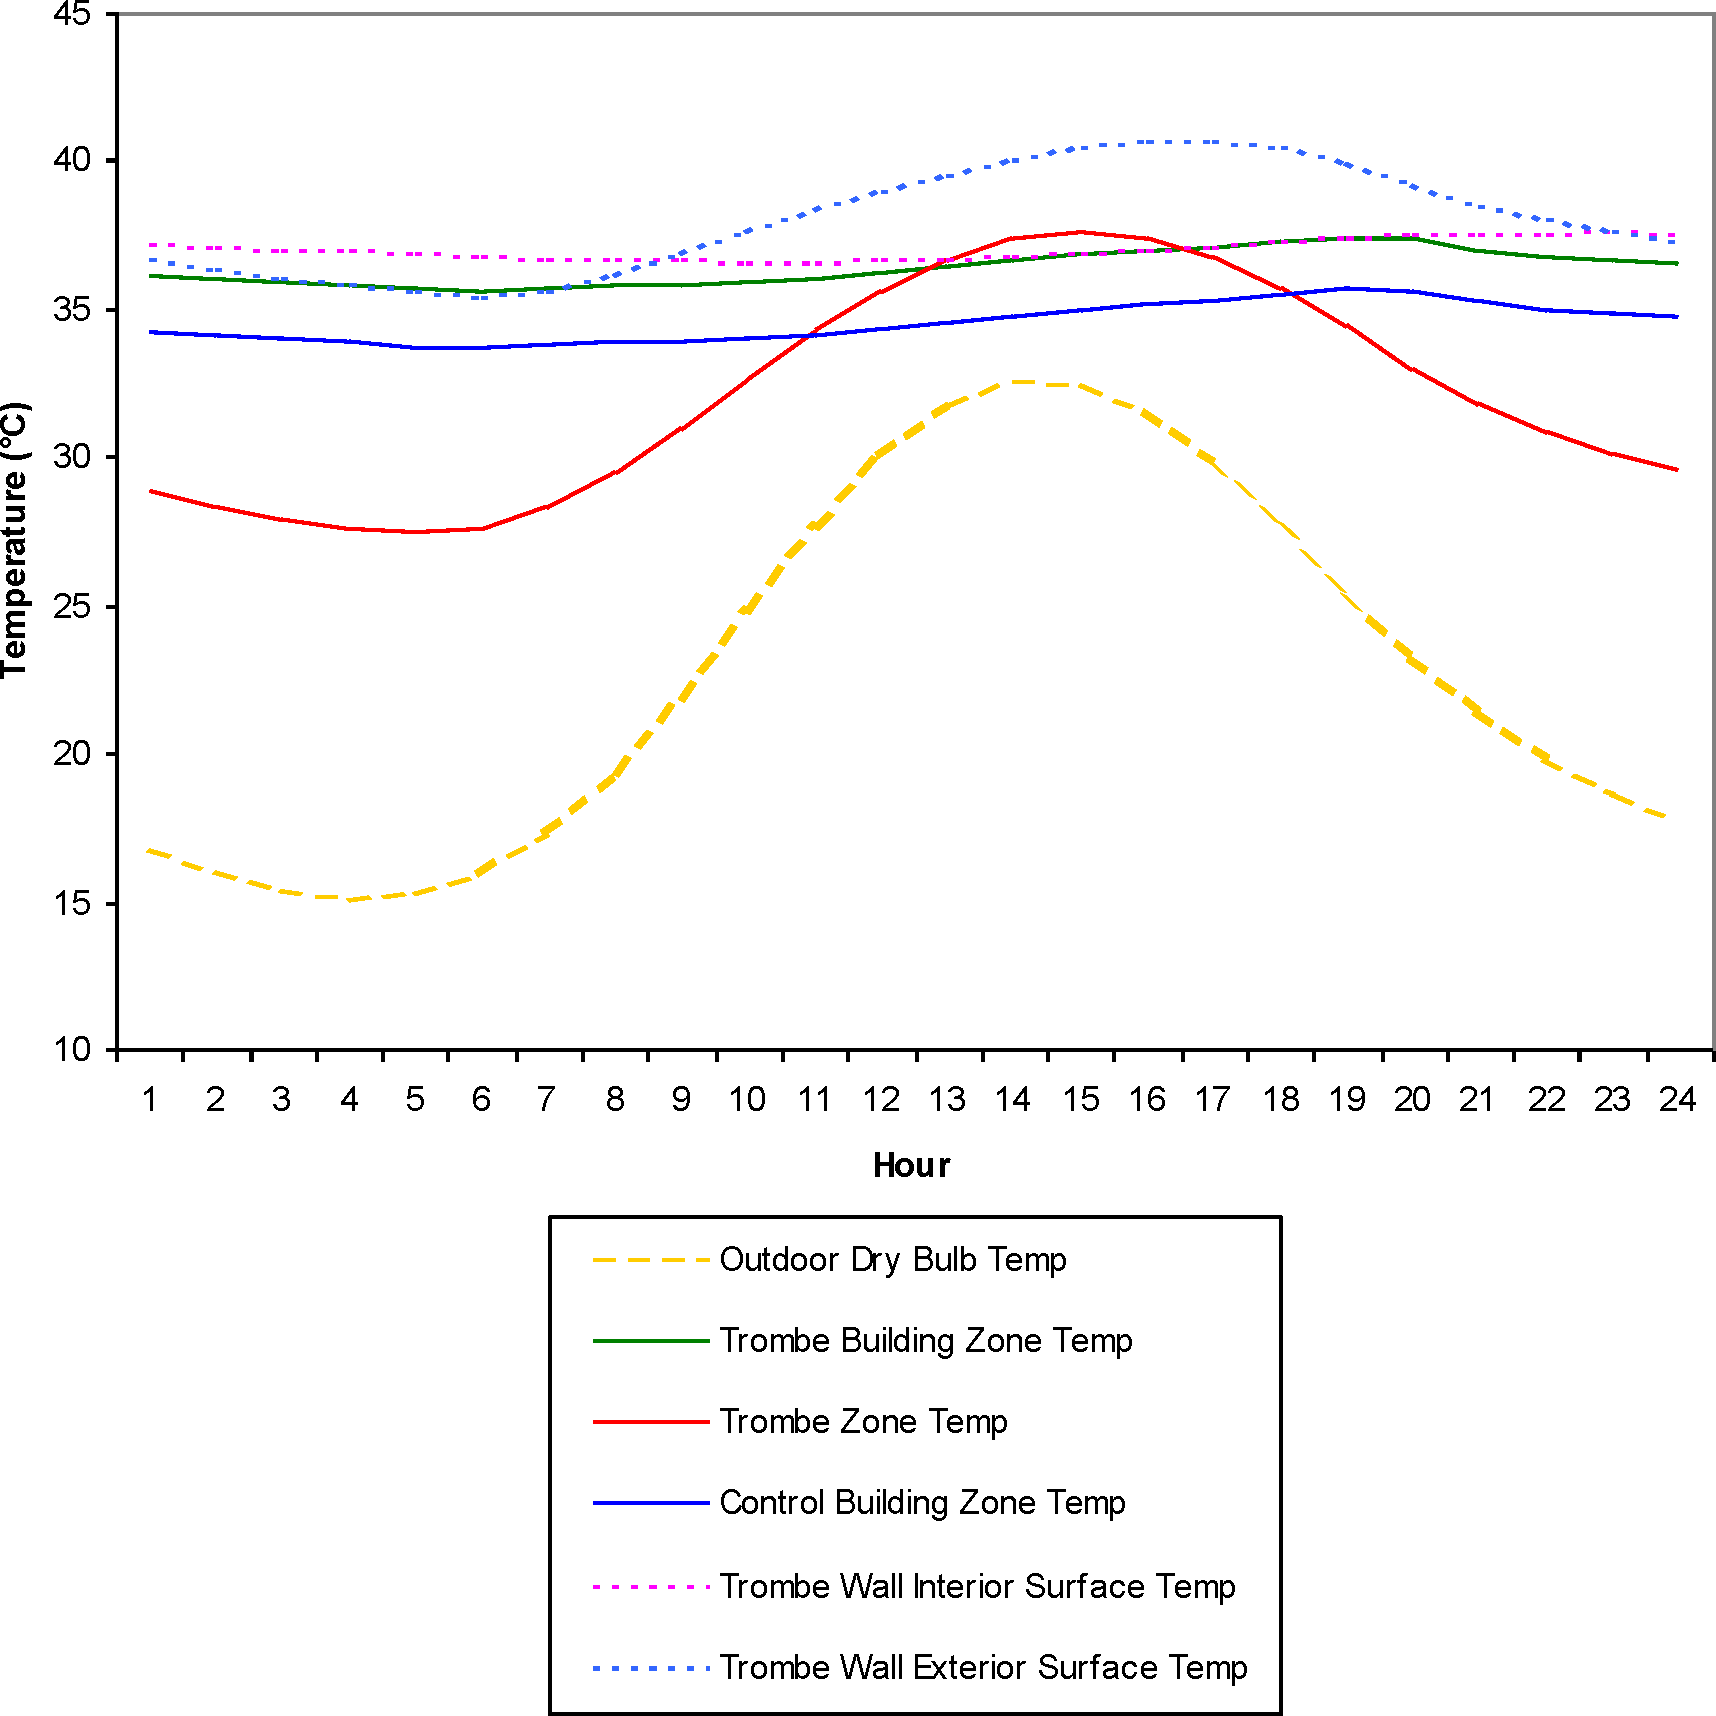
\includegraphics[width=0.9\textwidth, height=0.9\textheight, keepaspectratio=true]{media/image6832.png}
\caption{Passive Trombe Wall Summer \protect \label{fig:passive-trombe-wall-summer}}
\end{figure}

\subsubsection{References}\label{references-047}

Ellis, Peter G.~ 2003.~ \emph{Development and Validation of the Unvented Trombe Wall Model in EnergyPlus}, Master's Thesis, University of Illinois at Urbana-Champaign.

ISO 15099.~ 2000.~ ``Thermal Performance of Windows, Doors, and Shading Devices-Detailed Calculations''.~ International Standards Organization, Draft, July 18, 2000.

\subsection{Active Trombe Wall}\label{active-trombe-wall}

The active Trombe wall is the same as the passive Trombe wall with the addition of a simple fan system to circulate air between the Trombe zone and the main zone.~ The fan is scheduled to operate only during winter daylight hours to improve the heat transfer from the Trombe zone.

As with the passive Trombe wall, there is no EnergyPlus object for the active Trombe wall; it is simulated using a collection of other EnergyPlus objects.~ Like the passive Trombe wall, the active Trombe wall uses a narrow zone coupled to the main zone with interzone partitions.~ However, the unique part of the active Trombe wall is that the Trombe zone is used to define a zone supply plenum object which allows the Trombe zone to be integrated into the air system.~ A constant volume fan is the main component of the air system.~ To make the zone connections, the Direct Air component is used.

For the active Trombe wall, there is no built-in algorithm for calculating the correct convection coefficients due to forced convection on the inside of the cavity walls.~ One approach is to use the SurfaceProperty:ConvectionCoefficients object to schedule coefficients that have been determined beforehand by the user.

\subsubsection{Input File}\label{input-file-1}

An input file (ActiveTrombeWall.idf) is provided to demonstrate a sample active Trombe wall implementation.~ The building and Trombe wall in this file are identical to the ones described above for PassiveTrombeWall.idf.~ However, this input file adds a system in the form of a low flow rate (0.1 m\(^{3}\)/s) constant volume fan and the necessary duct connections.~ The fan is scheduled to operate October through March from 10 AM to 8 PM.

\subsubsection{Results}\label{results-1}

The resulting temperature profile for the winter design day is plotted below.~ The plot for the summer design day is not shown because it is identical to Figure~\ref{fig:passive-trombe-wall-summer} above since the fan is not scheduled to operate in the summer.

\begin{figure}[hbtp] % fig 310
\centering
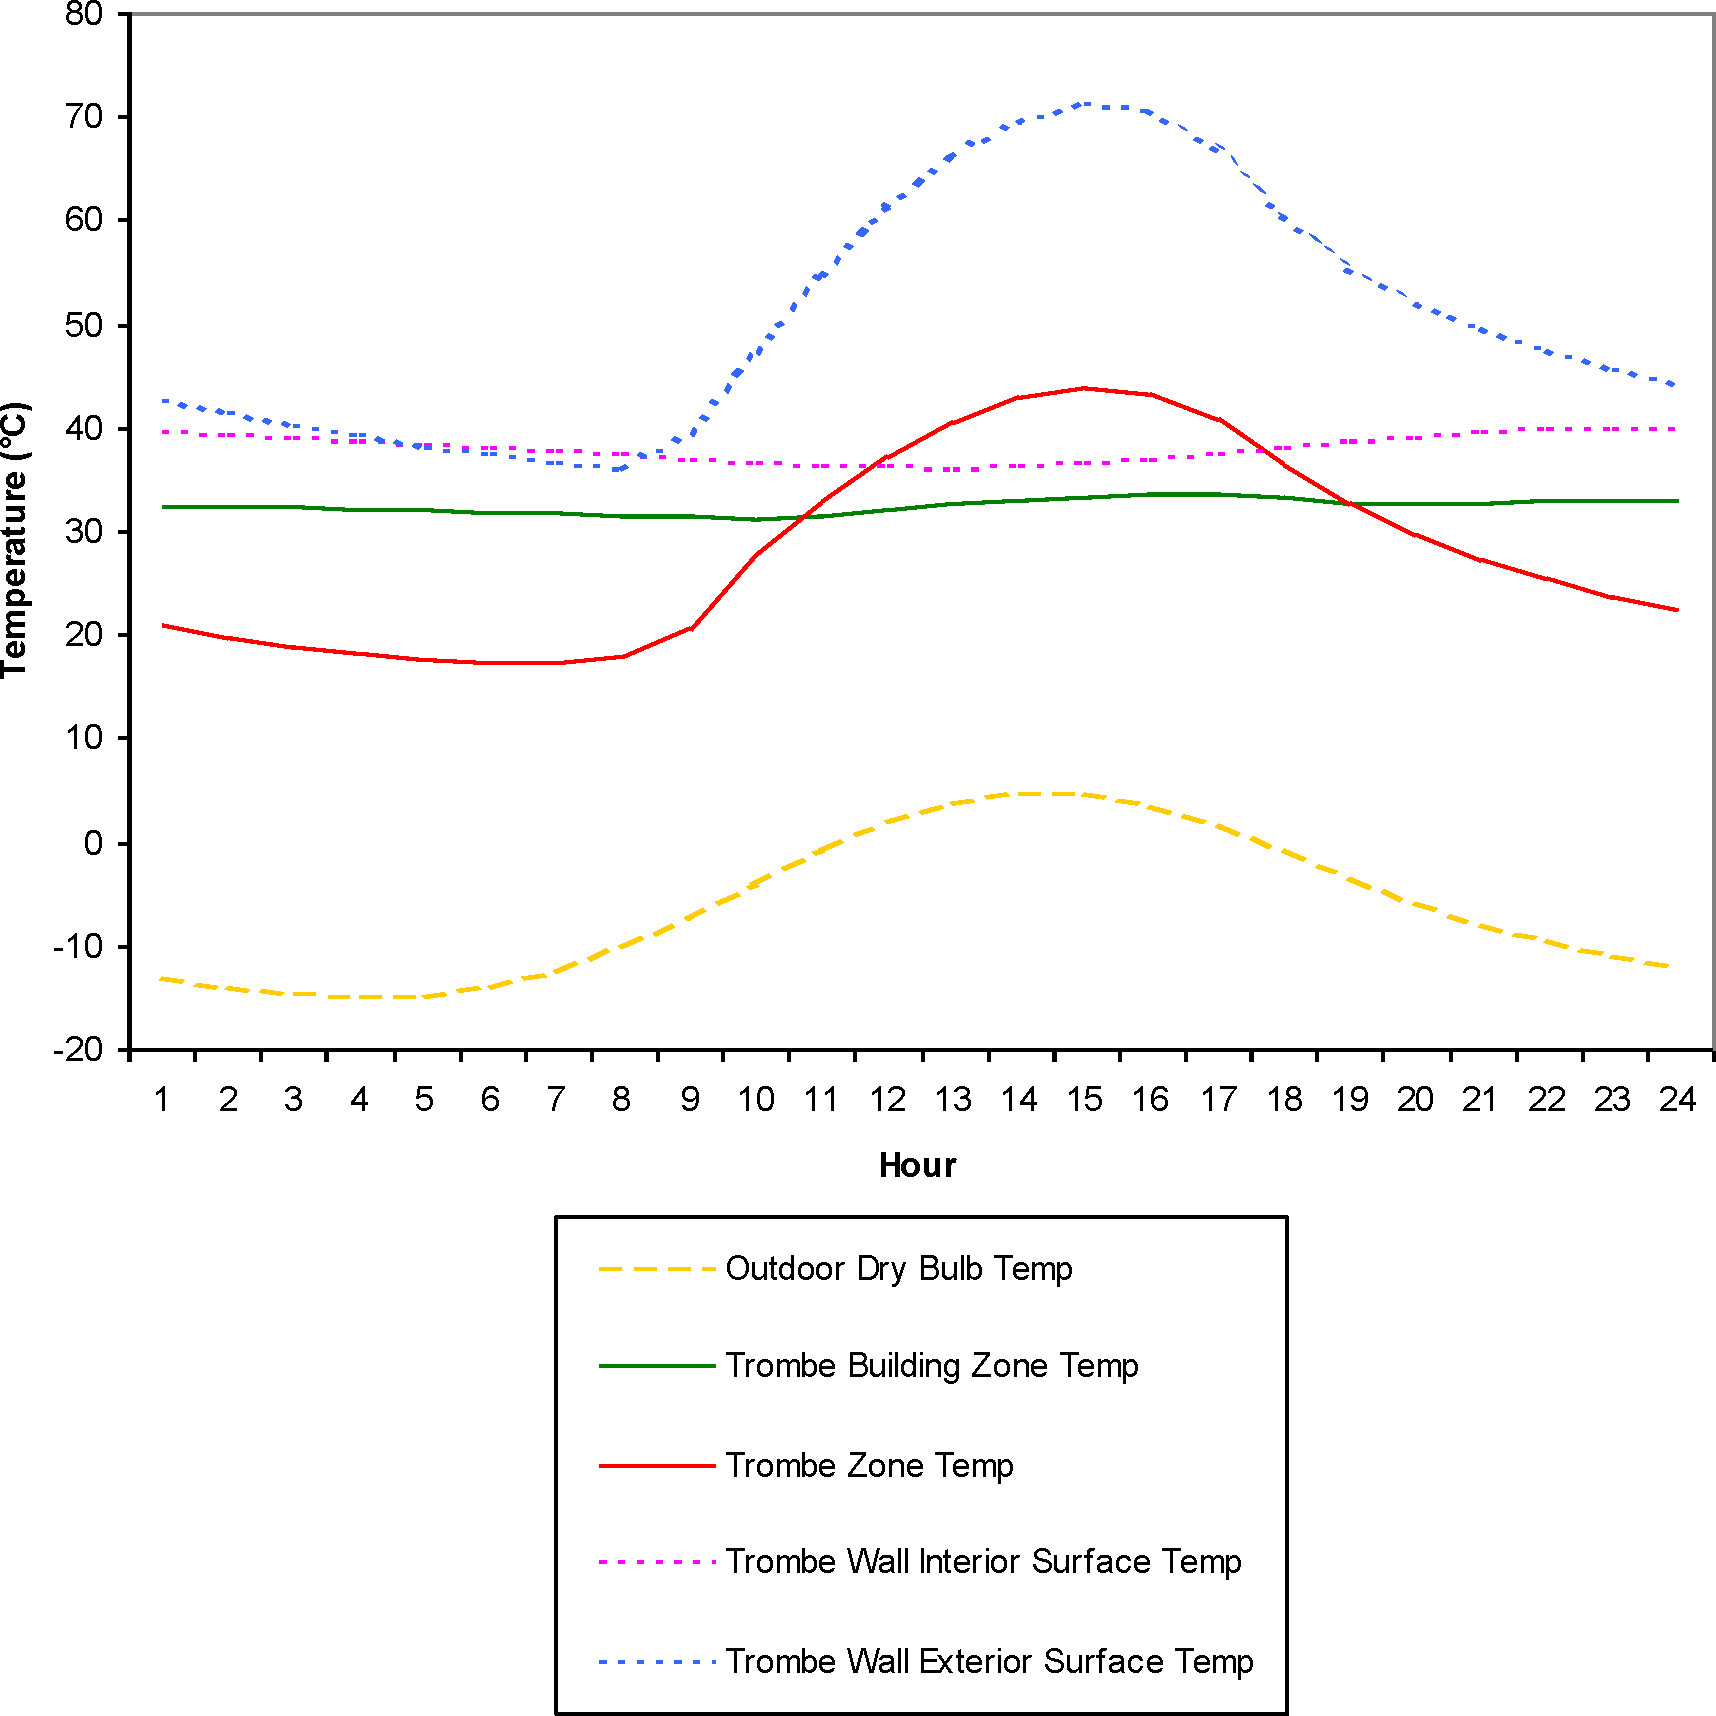
\includegraphics[width=0.9\textwidth, height=0.9\textheight, keepaspectratio=true]{media/image6833.png}
\caption{Active Trombe Wall Winter \protect \label{fig:active-trombe-wall-winter}}
\end{figure}
